% Template for IGARSS-2018 paper; to be used with:
%          spconf.sty  - LaTeX style file, and
%          IEEEbib.bst - IEEE bibliography style file.
% --------------------------------------------------------------------------
\documentclass{article}
\usepackage{spconf,amsmath,epsfig,graphicx,amsfonts}
\usepackage{subcaption}

% Example definitions.
% --------------------
\def\x{{\mathbf x}}
\def\L{{\cal L}}

% Title.
% ------
\title{Unsupervised Sequential Classification of MODIS Time-Series}
%
% Single address.
% ---------------
\name{T.L. Grobler$^{\dagger}$, W. Kleynhans$^{\star}$ and B.P. Salmon$^{\ddagger}$}
\address{$\dagger$Dept of Mathematical Sciences, Computer Science Division, Stellenbosch University,\\ Private Bag X1, 7602 Matieland, South Africa\\
$\star$Department of Electrical, Electronic and Computer Engineering University of Pretoria,\\
Pretoria 0002, South Africa\\
${\ddagger}$School of Engineering, University of Tasmania,
Hobart, TAS 7001, Australia}
%
% For example:
% ------------
%\address{School\\
%	Department\\
%	Address}
%
% Two addresses (uncomment and modify for two-address case).
% ----------------------------------------------------------
%\twoauthors
%  {A. Author-one, B. Author-two\sthanks{Thanks to XYZ agency for funding.}}
%	{School A-B\\
%	Department A-B\\
%	Address A-B}
%  {C. Author-three, D. Author-four\sthanks{The fourth author performed the work
%	while at ...}}
%	{School C-D\\
%	Department C-D\\
%	Address C-D}
%
\begin{document}
%\ninept
%
\maketitle
%
\begin{abstract}
In this paper we present a hypertemporal unsupervised sequential classification algorithm.  
We illustrate the usefulness of this algorithm at the hand of a case study. For our case study, we consider a Moderate Resolution Imaging Spectroradiometer dataset containing two land cover classes, namely natural vegetation and settlement. For the 
case study we considered in this paper, the proposed sequential classification approach perfomred on average 1.33 times better than conventional $k$-means.
\end{abstract}
%
\begin{keywords}
Gaussian Mixture Model (GMM), sequential detection, unsupervised, SPRT (Sequential Probability Ratio Test) and remote sensing.
\end{keywords}
%

\section{Introduction}
\label{sec:intro}
A remote sensing time-series is hypertemporal if its observational cadence is every few days. Clustering unlabelled hypertemporal remote sensing time-series can be a very useful first step in the analysis thereof. The algorithm which is arguably the most widely used approach to accomplish this task is the $k$-means algorithm \cite{viovy2000}. On the other hand, Gaussian Mixture Models (GMMs) are not often used for the clustering of hypertemporal remote-sensing time-series.

Skakun et al. used a GMM and NDVI (Normalized Difference Vegetation Index) time-series to discriminate winter crops from other crops (spring and summer) \cite{skakun2017}. The approach suggested by Skakun et al., although hypertemporal, does not fully exploit the temporal information contained witin the NDVI time-series it employs (it uses quantities derived form the raw time-series instead of the raw time-series itself).

In this paper, we propose a novel unsupervised sequential algorithm to cluster MODIS (Moderate Resolution Imaging Spectroradiometer) time-series. A sequential algorithm can process observations as they are received (it is an online algortihm). As our proposed approach is sequential, it is a hypertemporal technique per definition.
A supervised sequential classification algorithm which could discriminate 
between vegetation and settlement MODIS pixels was proposed in \cite{ackermann2011t,grobler2012c}. Grobler et al. used the Sequential Probability Ratio Test (SPRT) and a time-varing model which was constructed in a supervised manner to perform this task. 
The approach we present in this paper uses the SPRT algorithm and a time-varying model which we construct by employing GMMs to cluster MODIS time-series (i.e. in an unsupervised manner).

We start the paper by introducing the dataset we used to test the efficacy of our proposed algorithm. We present the GMM algorithm and our unsupervised sequential algorithm in Section~\ref{sec:GMM} and 
Section~\ref{sec:sprt}, respectively. We end our paper with some results and a conclusion.
\section{Data Description}
\label{sec:data}
The dataset that we use contains eight years worht of MODIS MCD43A4 BRDF (Bidirectional Reflectance Distribution Function) corrected 500 m land surface
data (925 MODIS pixels which correspond to approximately 230 km$^2$). The study area from which this data was obtained is the Gauteng province of South Africa. The dataset contain seven time-series which correspond to the 
MODIS land bands. Each time-series consist of 368 observations. The temporal cadence of the data is 45 observations per year. We considered only two landcover classes, settlement and vegetation. 
Vegetation MODIS pixels (592) contain more than 90\% vegetation, while settlement pixels (333) consist of more than 50\% buildings. We selected MODIS pixels that according to Système Probatoire d’Observation de la Terre (SPOT) images had the appropriate percentage land cover type in a MODIS pixel and did not change from 2000 to 2008.
In this paper we regarded the data associated with each year as new a new separate observations of either settlement of vegetation pixels. The final datamatrix $\mathbf{X}$, therefore, has the following dimensions (7400,45,7). The first dimension
indicates the number of observations we have, the second dimension represents the number of time-steps that we have, and the final dimension tells us the number of 
spectral bands we are considering.

\section{Gaussian Mixture Models}
\label{sec:GMM}
Let $\mathbf{Y}$ denote an $N\times M$ dataset. The dataset $\mathbf{Y}$ contains $N$ observations. Each observation $\mathbf{y}$ consist of $M$ features. Let us further assume 
that $\mathbf{Y}$ can be modelled as a $k$-component GMM:
\begin{equation}
P(\mathbf{y}|\boldsymbol{\theta})=\sum_{j=1}^k \pi_j \mathcal{N}(\mathbf{y}|\mathbf{u}_j,\mathbf{\Sigma}_j),
\end{equation}
where $\pi_j$ denotes the prior probability of the $j$-th Gaussian component, $\mathbf{u}_j$ denotes the mean and $\mathbf{\Sigma}_j$ denotes the covariance matrix associated with the $j$-th Gaussian component. Moreover,
$\mathcal{N}(\mathbf{y}|\mathbf{u},\mathbf{\Sigma})$ denotes a Gaussian density with a mean vector $\mathbf{u}$ and a covariance matrix $\mathbf{\Sigma}$. The symbol $\boldsymbol{\theta}$ denotes the set of all all 
model parameters.
We can determine the model parameters using the Expectation Maximization algorithm:
\begin{enumerate}
 \item Initialize $\boldsymbol{\theta}$. One possibility is to use the $k$-means algorithm.
 \item \textbf{E-Step}. Compute the responsibilities:
 \begin{equation}
  \gamma_{nj} = \frac{\pi_j\mathcal{N}(\mathbf{y}_n|\mathbf{u}_j,\mathbf{\Sigma}_j)}{\sum_{i=1}^{k}\pi_i\mathcal{N}(\mathbf{y}_n|\mathbf{u}_i,\mathbf{\Sigma}_i)}
 \end{equation}
 \item \textbf{M-step}. Compute the model parameters:
 \begin{eqnarray}
  \mathbf{u}_j &=& \frac{1}{N_j} \sum_{n=1}^{N} \gamma_{nj}\mathbf{y}_n\\
  \mathbf{\Sigma}_j &=& \frac{1}{N_j} \sum_{n=1}^{N} \gamma_{nj} (\mathbf{y}_n-\mathbf{u}_j)(\mathbf{y}_n-\mathbf{u}_j)^T\\
  \pi_j &=& \frac{N_j}{N}
 \end{eqnarray}
 where $N_j = \sum_{n=1}^N \gamma_{nj}$.
 \item Iterate from step two, until parameter convergence.
\end{enumerate}


\section{Sequential Probability Ratio Test}
\label{sec:sprt}
%At the start of the analysis the MODIS data set had the following dimensions (592,368,7). The first dimension is associated with the number of MODIS pixels, the second dimension indicates the number of observations, 
%while the third dimensions represents the number of spectral bands consdidered. The datset is then reshaped into a cube with the following dimensions (x,45,7), i.e. we treat each year of data as 
%a totally new observation. Let us denote this reshaped data set as $\mathcal{D}$.  Moreover, let $\mathbf{x}_{\mathbf{b}}$ denote a single MODIS pixel from $\mathcal{D}$ that contain only the time-series 
%associated with spectral bands $\mathbf{b}$. The dimension of $\mathbf{x}$ is therefore $(45,|\mathbf{b}|)$, where $|\cdot|$ denotes the lenght of its operand. We can now build a statistical model for each two band combination for every time-step of the year using either a supervised or an unsupervised strategy.
%We considered two band combinations as we know that two-band derived indices, like NDVI (Normalized Difference Vegitation Index), achieve good results. 
Let $\mathbf{x}$ denote a MODIS pixel from the Gauteng dataset $\mathbf{X}$ (see Section~\ref{sec:data}). Each MODIS pixel $\mathbf{x}$ contain seven time-series; each time-series is associated with a spectral band and contain 45 observations.
We will use the subscript $t$ to denote a time-step index and the subscript $\mathbf{b}$ to denote a composite spectralband index. The superscript $c\in\{v~\textrm{(vegetation)},s~\textrm{(settlement)}\}$ acts as a labelling index. Grobler et al. showed, that the SPRT algorithm can be used to distinguish between settlement and vegetation MODIS pixels if the underlying time-varying model of the two classes are known \cite{grobler2012c}. 
Let, $q_{t,\mathbf{b}}^c$ denote a density which accurately represents the data associated with class $c$, spectral bands $\mathbf{b}$ and time-step $t$. The aforementioned time-varying 
model is expressed mathematically as: $\{q_{t,\mathbf{b}}^c\}_{t=1,2,\cdots,45}$.
For each unlabelled MODIS pixel $\mathbf{x}_{\mathbf{b}}$ we can then compute the following scalar quantity: 
\begin{equation}
S = \sum_{t=1}^{45} \ln \frac{q_{t,\mathbf{b}}^v(\mathbf{x}_{t,\mathbf{b}})}{q_{t,\mathbf{b}}^s(\mathbf{x}_{t,\mathbf{b}})}. 
\end{equation}
The unlabelled pixel $\mathbf{x}$ is then classified as $v$ if $S\geq 0$ and as $s$ otherwise. We can estimate  $\{q_{t,\mathbf{b}}^c\}_{t=1,2,\cdots,45}$ using either a supervised or an unsupervised 
approach. 

\subsection{Supervised Time-Varying Model}
\label{sec:sup_model}
Let $\mathbf{X}_{t,\mathbf{b}}^c$ represent all the data from $\mathbf{X}$ at time-step $t$, associated with spectral bands $\mathbf{b}$ and labbeled as $c$. We can now fit a Gaussian density 
to $\mathbf{X}_{t,\mathbf{b}}^c$; the dimension of which is determined by the number of spectral bands one considers. To accomplish this in practise we used the \texttt{mixture.GaussianMixture} class from \textsc{scikit-learn}. 
As we are creating separate time-varying models for $v$ and $s$ we set the \texttt{n\_components} input parameter of the aforementioned class's constructor to 1. We then repeat the above procedure for each class and time-step and in 
doing so we build the required time-varying models. %The supervised time-varying models which were constructed using $\mathbf{b}=\{1,2\}$ is depicted in Figure~\ref{fig:time_vary_model}.

\subsection{Unsupervised Time-Varying Model}
Let $\mathbf{X}_{t,\mathbf{b}}$ represent all the data from $\mathbf{X}$ at time-step $t$ associated with spectral bands $\mathbf{b}$. We can now fit a two-component GMM to $\mathbf{X}_{t,\mathbf{b}}$ (as $\mathbf{X}$ contain only two classes). Again,
the dimension of this model is determined by the number of spectral bands one consides (see Section~\ref{sec:GMM}). We can repeat the above procedure for each time-step and in doing so 
build the required time-varying model (again this is accomplished in practise using \texttt{mixture.GaussianMixture} with \texttt{n\_components=2}). The only problem now is that the components of the mixture models will have been inconsistantly labelled accross time. There are many approaces one could use to assure 
that the components of the mixture model are consistently labelled across time. The simplest approach would be to compute the sum of the euclidean distance between the means of 
the first and the second components of the GMM at $t$ and $t-1$; and to compare this sum with the sum of the euclidean distance between the means of the first component of the GMM at time $t$ and 
the second component of the GMM at time $t-1$; and the euclidean distance between the mean of the second component of the GMM at time $t$ and the mean of the first component of the GMM at time $t-1$. If the latter sum is 
larger than the former the labels of the components at $t$ should be swopped, otherwise the labels should be left as is. This relabelling procedure should be repeated for each time-step $t$.

In this paper, however, we labelled our unsupervised time-varying model by employing the supervised time-varying models mentioned in Section~\ref{sec:sup_model}. We followed this approach, because 
we wanted to quantify the optimal performance of the unsupervised time-varying model we constructed. At each time-step $t$ we 
determined whether the sum of the euclidean distance between the mean of our first GMM component and the mean of the density belonging to our settlement model and the euclidean distance 
between the mean of our second GMM component and the mean of the density belonging to our vegetation model; was smaller than the sum of the euclidean distance between the mean of our first GMM coponent and the mean of the density 
belonging to our vegetation model and the euclidean distance between the mean of our second GMM component and the mean of the density of our settlement model. If this was the case then our first GMM component 
was labelled as belonging to the settlement class and the second component was labbelled as belonging to the vegetation class. If this was not the case then 
the reverse labels were assigned. The supervised and the unsupervised time-varying models which were constructed using $\mathbf{b}=\{1,2\}$ is depicted in Figure~\ref{fig:time_vary_model}.

% density contained in the vegetation model well as our v than to the density 
% contained in our vegetation model.
% assigned the components of the GMM at that time-step 
% to the density  closest to it. 
% 
% approach as we were interested i We used our supervised 
% model to label our unsupervised model (the GMM component at time-step $t$ which was closest to the settlement density at time-step $t$  was identified as being 
% cluster was


% We first solved the following 
% optimization problem:
% \begin{equation}
% \inf_{\mathbf{c}\in\{\{s,v\},\{v,s\}\}} \|\mathbf{u}_{t,\mathbf{b}}^{0}-\tilde{\mathbf{u}}_{t,\mathbf{b}}^{c_0}\| + \|\mathbf{u}_{t,\mathbf{b}}^{1}-\tilde{\mathbf{u}}_{t-1,\mathbf{b}}^{c_1}\|,  
% \end{equation}
% with $\tilde{\mathbf{u}}_{t,\mathbf{b}}^{c} = \mathbb{E}_t[\mathbf{X}_{t,\mathbf{b}}^c]$. Then, if $c_0 = s$ then the component   

\begin{figure}[h!]
\begin{minipage}[b]{.47\linewidth}
  \centering 
  \centerline{\epsfig{figure=11.pdf,width=4.0cm}}
  %\vspace{1.5cm}
  \centerline{(a) $t=11$}\medskip
\end{minipage}
\hfill
\begin{minipage}[b]{0.47\linewidth}
  \centering
  \centerline{\epsfig{figure=22.pdf,width=4.0cm}}
  %\vspace{1.5cm}
  \centerline{(b) $t=22$}\medskip
\end{minipage}

\begin{minipage}[b]{.47\linewidth}
  \centering 
  \centerline{\epsfig{figure=33.pdf,width=4.0cm}}
  %\vspace{1.5cm}
  \centerline{(c) $t=33$}\medskip
\end{minipage}
\hfill
\begin{minipage}[b]{0.47\linewidth}
  \centering
  \centerline{\epsfig{figure=44.pdf,width=4.0cm}}
  %\vspace{1.5cm}
  \centerline{(d) $t=44$}\medskip
\end{minipage}
\caption{The 95\% confidence intervals of the time-varying models associated with the settlement (red) and the vegetation (green) class which were constructed using either a supervised (solid) or an unsupervised approach at time-step 11, 22, 33 and 44 (constructed 
for band 1 and band 2). The details of exactly how these models were constructed is discussed in Section~\ref{sec:sprt}.}
\label{fig:time_vary_model}
\end{figure}

\section{Results}
In this section we present the performance results of the supervised and the unsupervised sequential classification algorithms we presented in Section~\ref{sec:sprt}.
Note, the data which was used by the SPRT algorithm to generate the classification results we present here was the same data we used to construct the time-varying models that are required by the SPRT algorithm.  
Furhtermore, we restrict our analysis to two band combinations (we decided on two band combinations as the time-varying model 
one can construct for two band combinations can be nicely visualized). We also compare these two approaches with two other more conventional clustering approaches, which entails applying the $k$-means and GMM algorithms to the entire time-series directly.
The results are depicted in Figure~\ref{fig:results}. The average classification accuracy of the supervised and the unsupervised sequential classification aproaches are 94\% and 80\%, repspectively. Which is 
as expected; a supervised approach will outperform an unsupervised approach. When we directly apply the $k$-means and the GMM algorithm to the time-series we obtain 
an average classification accuracy of 60\% and 51\%. The $k$-means algorithm, therefore, outperforms the GMM approach. Note, that the sequential unsupervised approach which uses 
GMMs to construct its underlying time-varying model, however, outperforms conventional $k$-means. 

\begin{figure*}[h] 
  \begin{subfigure}[b]{0.49\linewidth}
    \centering
    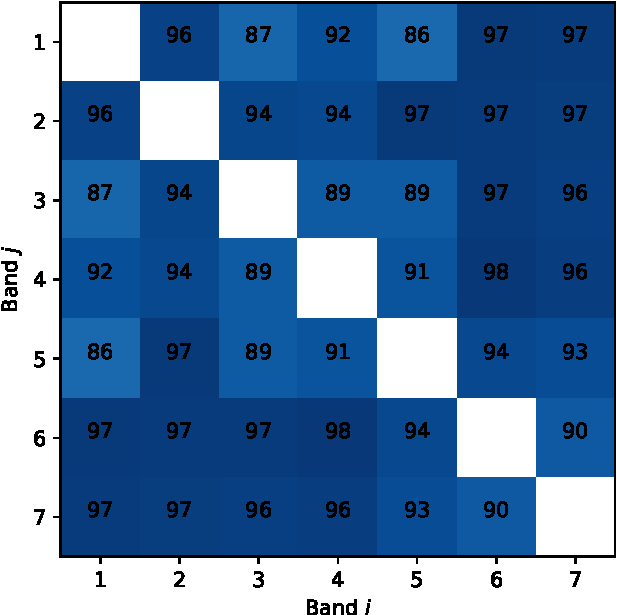
\includegraphics[width=0.85\linewidth]{sup-crop.pdf} 
    \caption{Logarithm applied} 
    \label{fig7:a} 
    %\vspace{4ex}
  \end{subfigure}%% 
  \begin{subfigure}[b]{0.49\linewidth}
    \centering
    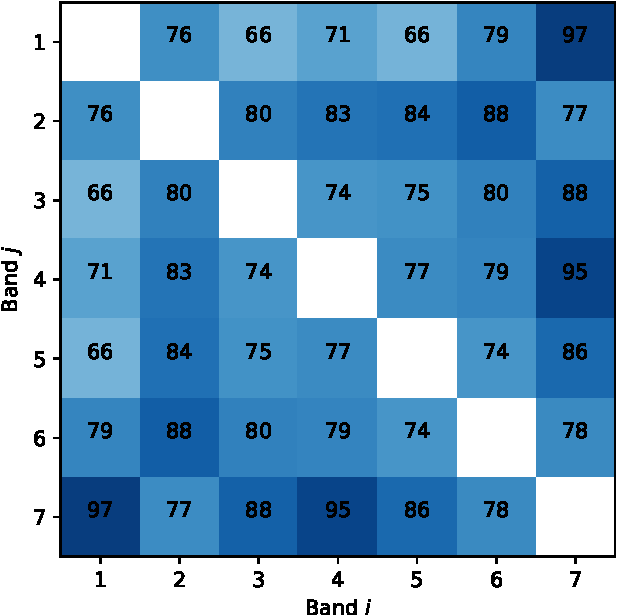
\includegraphics[width=0.85\textwidth]{un-crop.pdf} 
    \caption{Binary segmented image} 
    \label{fig7:b} 
    %\vspace{13ex}
    \end{subfigure} 
  \begin{subfigure}[b]{0.49\linewidth}
    \centering
    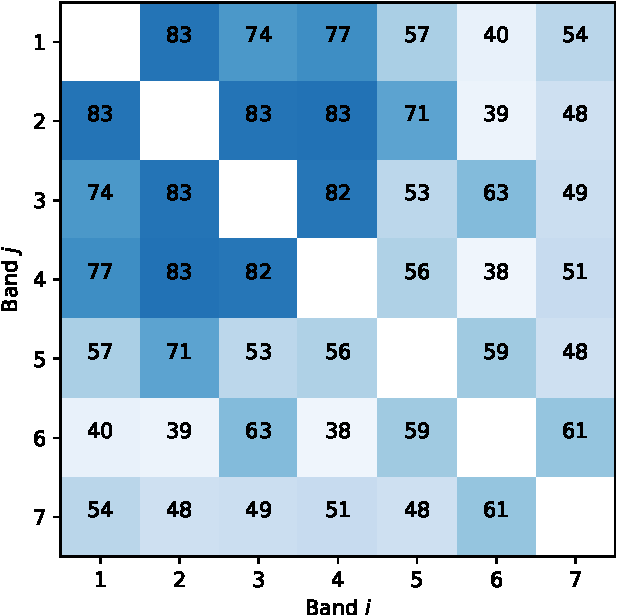
\includegraphics[width=0.85\textwidth]{kmeans-crop.pdf} 
    \caption{Hough Transform} 
    \label{fig7:c} 
  \end{subfigure}%%
  \begin{subfigure}[b]{0.49\linewidth}
    \centering
    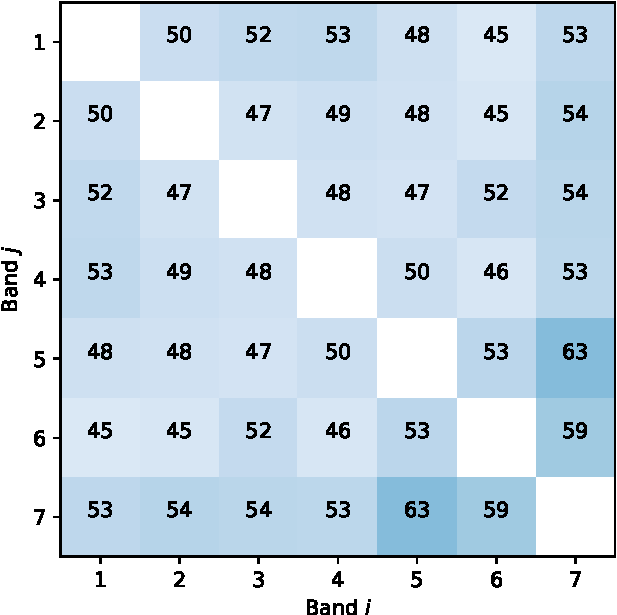
\includegraphics[width=0.85\textwidth]{gmm-crop.pdf} 
    \caption{Segmented image} 
    \label{fig7:d} 
  \end{subfigure} 
  \caption{c}
  \label{fig7} 
  \caption{The classification accuracy results of the supervised (top left) and the unsupervised (top right) sequential classification approach presented in Section~\ref{sec:sprt} are depicted in this figure. The classification
  accuracy results obtained by applying $k$-means (bottom left) and GMM (bottom-right) to the time-series directly are also depicted in the above figure. The supervised approach outperforms the 
  unsupervised approach as is expected. Note, the unsupervised sequential approach, however, outperforms traditional $k$-means.}
  \label{fig:results}
\end{figure*}

\section{Conclusion}
\label{sec:ref}
We presented a hypertemporal label agnostic sequential classification algorithm. For the case study presented in this paper, the proposed algorithm 
outperforms traditional $k$-meanse.

%List and number all bibliographical references at the end of the paper.  The references can be numbered in alphabetic order or in order of appearance in the document.  When referring to them in the text, type the corresponding reference number in square brackets as shown at the end of this sentence \cite{C2}.

% References should be produced using the bibtex program from suitable
% BiBTeX files (here: strings, refs, manuals). The IEEEbib.bst bibliography
% style file from IEEE produces unsorted bibliography list.
% -------------------------------------------------------------------------
\bibliographystyle{IEEEbib}
\bibliography{strings,refs}

\end{document}
